\documentclass[11pt, oneside]{article}   	% use "amsart" instead of "article" for AMSLaTeX format
\usepackage{geometry}                		% See geometry.pdf to learn the layout options. There are lots
\geometry{letterpaper}                   		% ... or a4paper or a5paper or ... 
%\geometry{landscape}                		% Activate for for rotated page geometry
%\usepackage[parfill]{parskip}    		% Activate to begin paragraphs with an empty line rather than an indent
\usepackage{graphicx}				% Use pdf, png, jpg, or eps§ with pdflatex; use eps in DVI mode
								% TeX will automatically convert eps --> pdf in pdflatex		
\usepackage{amssymb}
\usepackage{amsmath}
\usepackage{graphicx}


\title{Project Proposal}
\author{Ibrahim Taher and Forrest Hooton}
%\date{}							% Activate to display a given date or no date

\begin{document}
\maketitle
%\section{}
%\subsection{}

\textbf{Abstract.}

Convolutional neural networks have demonstrated the capacity to excel at object recognition. However, it fails at generating sequences of words. We aim to accomplish that by adding a second deep learning algorithm into the model, recurrent neural networks. We aim to develop a model that uses the spatial properties derived from a convultional neural network to create sequences of words using the recurrent neural network. The model will be trained and tested using the Microsoft COCO 2014 dataset amd the model performance will be evaluating using the BLEU error metric.

\vspace{5mm}
\textbf{Introduction.}

In the last decade, we have experienced exponential growth in terms of images on the internet. With these pictures come context, such as the scenery, events and sentiment. Often times this context is represented through the use of a human generated caption. These captions can range from simple descriptions ("There is a cat on a suitcase") to complex understandings of the context ("The sad man eats his sandwich.") These captions can be used to augment several use cases such as helping the visually impaired understand images or generating better search queries for images.

There has been ground-breaking work regarding annotating images with simple identifiers. Take for instance the following image

\vspace{5mm}
\begin{center}
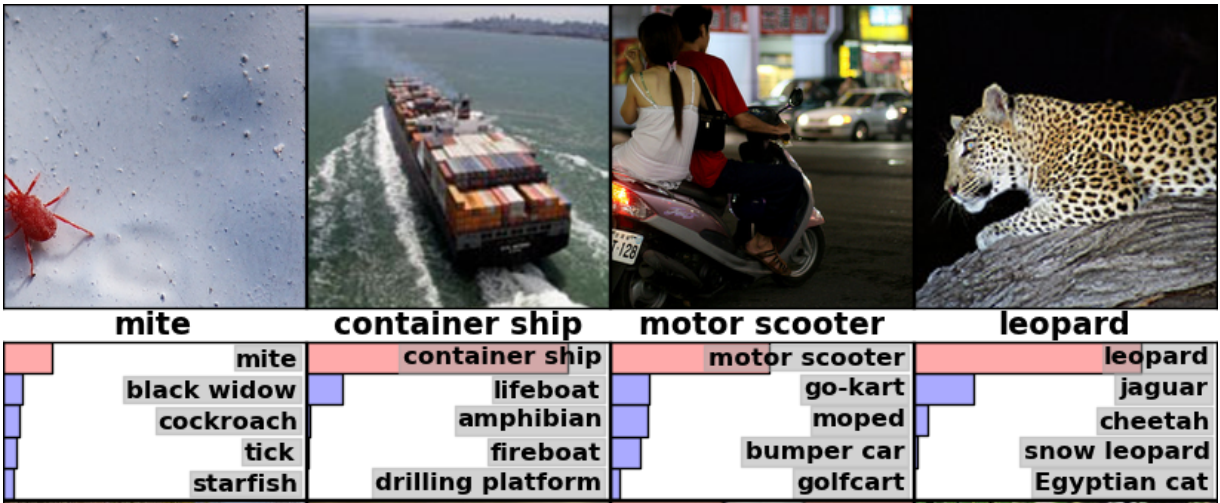
\includegraphics[scale=0.19]{figures/AlexClassification.png}
\end{center} 
 
\vspace{5mm}
These are a few examples of the advances that have been made in simple image recognition using convolutional neural networks. The model uses probabilities generated from a softmax function to determine what image might be. This transformation involves several layers that use techniques such as convolution, pooling and filtering to gather important features of the image. These techniques aim to exploit the spatial properties of the data and accomplish dimensionality reduction in order to identify objects.

Since convolutional neural networks are best for using spatial properties to generate simple outputs, another algorithm is needed to use information from the CNN to generate a caption. Recurrent neural networks allow for the generation of sequences using any variable input. The goal is to use the vector generated before the caption in a classic convolutional neural network and pipe that in as an input to the recurrent neural network. As a result, the overarching model architecture might resemble the following:

\vspace{5mm}
\begin{center}
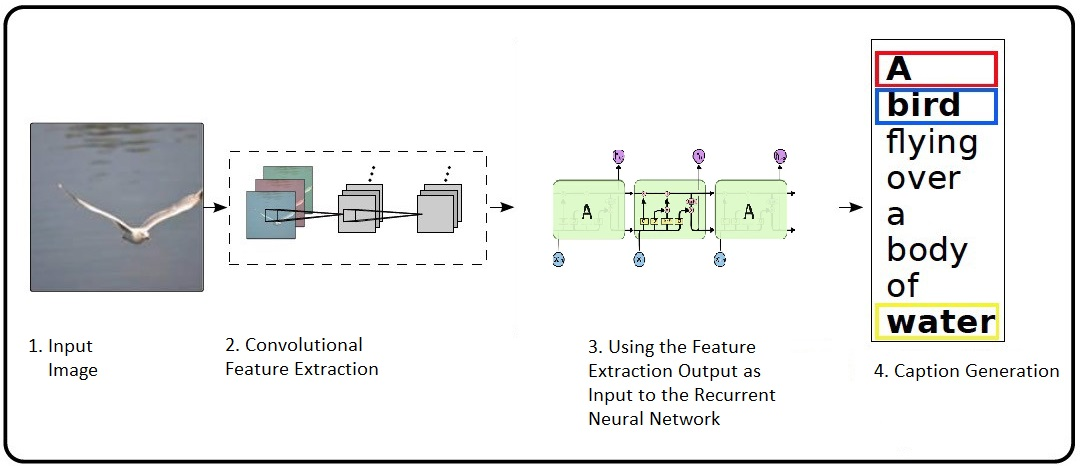
\includegraphics[scale=0.5]{figures/cnnrnnmodel.jpeg}
\end{center}

In order to create a robust model we will tune several parameters that are involved in the convolutional feature extraction. These include feature size and number of features (features being the representative chunks of an object we will use for classifying images) and window stride and size (how big will our windows on the image be and much will we move the window.) For both neural networks the number of neurons and layers and the learning rate will be tuned. Also, for truncated backpropogation (in order to determine weights) the number of epochs needed to do a backwards pass will need to be determined.

The data comes from the Microsoft COCO 2014 dataset, which includes several thousand images with associated captions. The dataset already comes pre-split with training and validation images but also comes with a testing set.

We plan to test our model using the BLEU error metric. The BLEU error metric is a method to evaluate the precision of a predicted caption.

\begin{center}
	$BLEU_{(a,b)} = \frac{\sum_{w_n \in a} min(c_a(w_n),max(c_{b_j}(w_n))}{\sum_{w_n \in a} c_a(w_n)}$
\end{center}

Where $a$ is a predicted caption, $b$ is a set of ground truth captions, $w_n$ is an n-gram and $c_x(y_n)$ is the count of n-gram $y_n$ in caption $c_x$.
\vspace{5mm}
\end{document}